\section{Contexte}

Une description plus détaillée de l'implantation de Linux peut être trouvée dans
\cite{UnderstandingTheLinuxKernel}.

\section{Rôle d'un système d'exploitation}
\section{Espace noyau, espace utilisateur}

\todo{OS = kernel ?}

Le système d'exploitation est l'interface logicielle entre le matériel et les
programmes qui vont s'exécuter sur un ordinateur. Pour une description détaillée
de son rôle typique, le lecteur pourra se référer à \cite{tanenbaum}.

Néanmoins on peut citer les rôles suivants :

\begin{itemize}
\item gestion des processus : un système d'exploitation peut permettre
  d'exécuter plusieurs programme à la fois. Il faut alors orchestrer ces
  différents processus et les séparer en terme de temps et de ressources
  partagées.
\item
  gestion de la mémoire : chaque processus, en plus du noyau, doit disposer d'un
  espace mémoire différent. C'est-à-dire qu'un processus ne doit pas pouvoir
  interférer avec un autre.
\item
  gestion des périphériques : le noyau étant le seul code à s'exécuter en mode
  privilégié, c'est lui qui doit communiquer avec les périphériques matériels.
\item
  abstractions : le noyau fournit au programmes une interface unifiée,
  permettant de stocker des informations de la même manière sur un disque dur ou
  une clef USB (alors que l'accès se déroulera de manière très différente en
  pratique). C'est ici que la notion arbitraire de fichier sera définie, par exemple.
\end{itemize}

\section{Cas de Linux}

Sous Linux, on retrouve cette séparation entre espace noyau et espace
utilisateur. Cette section décrit l'implémentation de cette séparation dans le
contexte suivant :

\begin{itemize}
\item l'architecture Intel x86
\item un système 32 bits
\item le noyau Linux
\end{itemize}

Sous d'autres architectures et d'autres systèmes d'exploitation, des mécanismes
similaires existent, et ces travaux peuvent sans doute s'y appliquer.

L'isolation est réalisée par le matériel. Ce document présente le cas d'un
système Intel 32 bits (x86), mais sous d'autres architectures des protections
similaires existent.

Le processeur permet d'exécuter des tâches selon plusieurs niveaux de privilège,
aussi appellés \emph{rings} : du \emph{ring} 3, le moins privilégié, jusqu'au
\emph{ring} 0, le plus privilégié. On peut configurer le processeur de manière à
ce que les instructions privilégiées (accès aux ports d'entrée/sortie...) ne
soient possibles qu'en \emph{ring 0}. Bien que 4 niveaux soient disponibles,
Linux n'utilise que les \emph{rings} 0 et 3.

Cela profite également au concept de mémoire virtuelle : comme différentes
tâches vont avoir une vue de la mémoire différente, on peut réserver une zone de
la mémoire aux tâches privilégiées.

\begin{figure}

\begin{tikzpicture}

\begin{scope}

  \path[clip] (-1, 0.8) rectangle (5, -0.8);

  \foreach \x/\c in { 4/20, 3/30, 2/40, 1/50, 0/60 }
  \draw[fill=black!\c] ($ (-2,0) + (\x,0) $) circle (2 cm);

\end{scope}

%\draw [<-] (3.5, 0) -- ++(0,-2) node {Applications};
%\draw [<-] (0, 0) -- ++(0,-2) node {Noyau};

\end{tikzpicture}


\caption{Les différents \emph{rings}. Seul le \emph{ring} 0 a accès au hardware
via des instructions privilégiées. Pour accéder aux fonctionnalités du noyau,
les programmes utilisateur doivent passer par des appels système.}

\label{fig:rings}
\end{figure}

\begin{figure}
\centering
\fbox{
  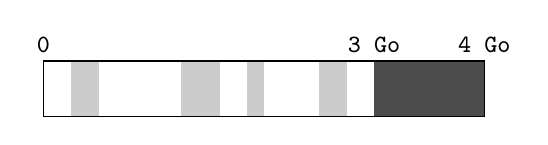
\begin{tikzpicture}
  [scale=0.7
  ,user/.style={fill=black!20}
  ,kernel/.style={fill=black!70}
  ]

  % Memory zone
  %
  % #1 - start
  % #2 - end
  % #3 - color
  \newcommand{\mzone}[3]{
    \path[#3] (#1,0) rectangle (#2,1);
  }

  % Address label
  %
  % #1 - x position
  % #2 - text
  \newcommand{\alabel}[2]{
    \path (#1,1) -- ++(0,0.3) node [pos=1] {\small \ttfamily #2};

  }

  % exec
  \mzone{0.5}{1}{user}

  % lib
  \mzone{2.5}{3.2}{user}

  % stack
  \mzone{3.7}{4}{user}

  % stack
  \mzone{5}{5.5}{user}

  % kernel
  \mzone{6}{8}{kernel}

  % contour
  \draw (0,0) rectangle (8,1);

  \alabel{0}{0}
  \alabel{6}{3 Go}
  \alabel{8}{4 Go}

\end{tikzpicture}

}

\caption{L'espace d'adressage d'un processus. En gris clair, les zones
accessibles à tous les niveaux de privilèges : code du programme, bibliothèques,
tas, pile. En gris foncé, la mémoire du noyau, réservée au mode privilégié.}

\label{fig:memmap}
\end{figure}

\section{Appels système}

Les programmes utilisateur s'exécutant en \emph{ring} 3, ils ne peuvent pas
contenir d'instructions privilégiées, et donc ne peuvent pas accéder directement
au matériel (c'était le but !). Pour qu'ils puissent interagir avec le système
(afficher une sortie, écrire sur le disque...), le mécanisme des appels système
est nécessaire. Il s'agit d'une interface de haut entre les \emph{rings} 3 et 0.
Du point de vue du programmeur, il s'agit d'un ensemble de fonctions C
"magiques" qui font appel au système d'exploitation pour effectuer des
opérations.

Prenons le cas de l'appel `getpid`, qui retourne le numéro de processus courant.
La bibliothèque C fournit une fonction du même nom :

\begin{Verbatim}
$ man getpid

GETPID(2)                  Linux Programmer's Manual                  GETPID(2)

NAME
       getpid, getppid - get process identification

SYNOPSIS
       #include <sys/types.h>
       #include <unistd.h>

       pid_t getpid(void);
       pid_t getppid(void);

DESCRIPTION

       getpid() returns the process ID of the calling process.  (This is often
       used by routines that generate unique temporary filenames.)
\end{Verbatim}

A priori, rien de différent d'une fonction implantée directement en C. Par un
processus détaillé ci-après, cette fonction va invoquer la fonction, suivante,
définie dans le noyau (\texttt{kernel/timer.c}) :

\begin{Verbatim}
SYSCALL_DEFINE0(getpid)
{
        return task_tgid_vnr(current);
}
\end{Verbatim}

Le mécanisme de couplage entre ces deux fonctions est le suivant :

  - la fonction de la libc place les arguments éventuels de l'appel système dans
    les registres.
  - un numéro identifiant l'appel système est placé dans \eax.
  - une interruption logicielle est déclenchée :
